% final draft
% todo: Interkapitel-Referenzen, Kontextgrafik


\chapter{Überblick über die empirische Untersuchung}
\label{cha:eval_ueberblick}

In diesem Kapitel wird ein Überblick über die in dieser Arbeit durchgeführte empirische Untersuchung gegeben. Dabei wird auf die einzelnen zu untersuchenden Aspekte, deren theoretische Grundlagen und die Durchführung der Untersuchung gegeben. Abbildung \ref{fig:img_Kontextgrafiken_k11} stellt dieses Kapitel und dessen Aufbau im Kontext der anderen inhaltlich vor- und nachgelagerten Kapitel dar.


\begin{figure}[htbp]
	\centering
		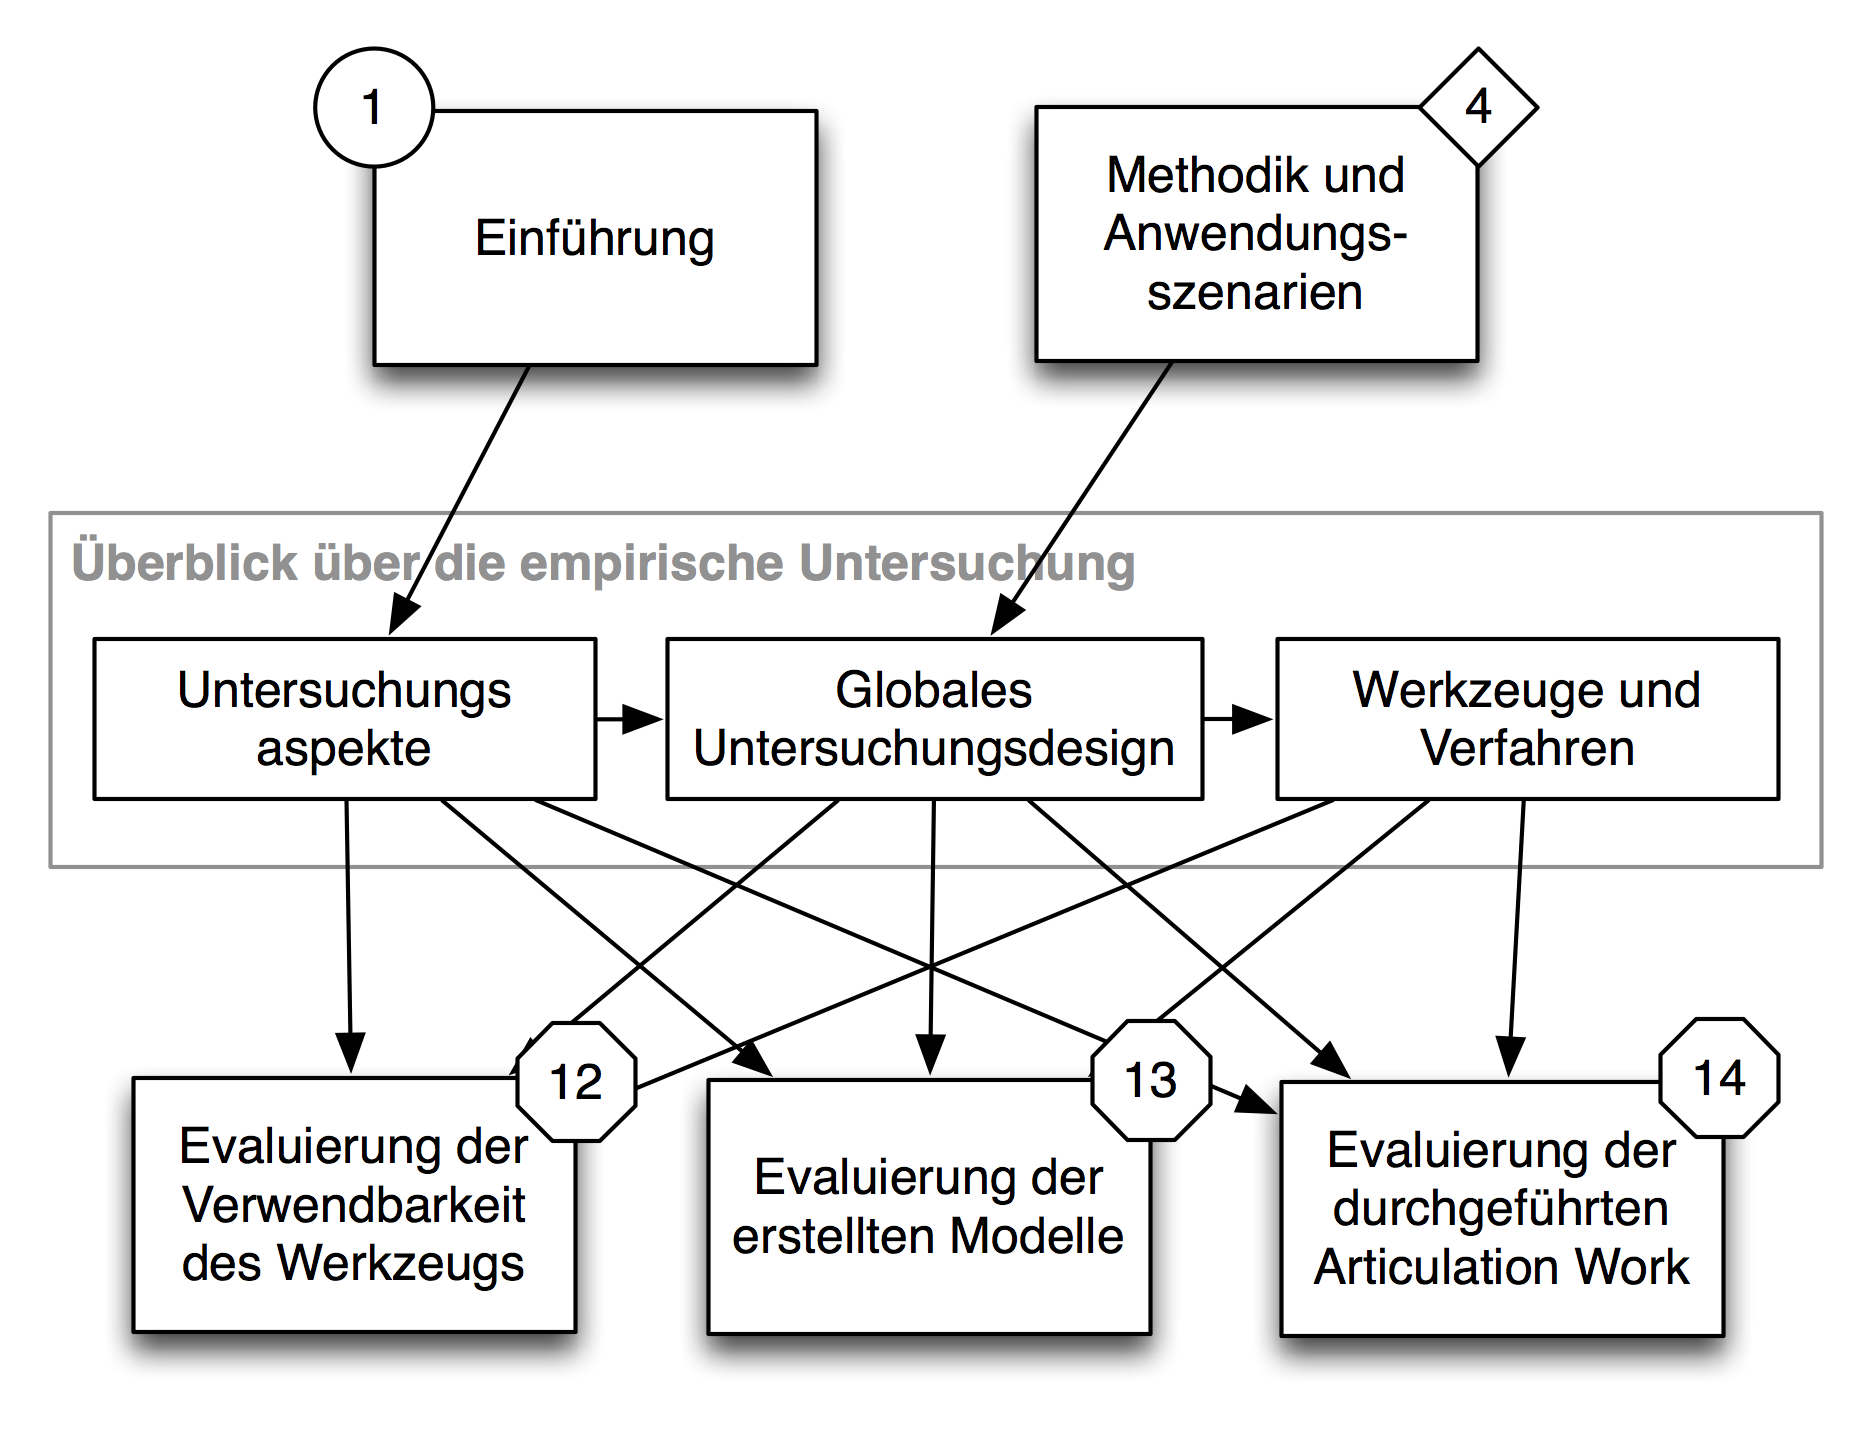
\includegraphics[scale=0.6]{img/Kontextgrafiken/k11.png}
	\caption{Kapitel „Überblick über die empirische Untersuchung“ im Gesamtzusammenhang}
	\label{fig:img_Kontextgrafiken_k11}
\end{figure}

Die im Rahmen der empirischen Evaluierung zu untersuchenden Aspekte sind Gegenstand des ersten Abschnitts. Neben einer wiederholenden grundlegenden Betrachtung werden hier die jeweiligen Untersuchungsfragen festgelegt. Eine nähere Betrachtung der einzelnen Aspekte, die Festlegung der Methodik und deren Operationalisierung im Rahmen des konkreten Untersuchungsdesigns erfolgt im Rahmen der übrigen Kapitel in diesem Teil der Arbeit.

Im zweiten Abschnitt wird ein Überblick über das globale Untersuchungsdesign gegeben. Auf Basis der zu evaluierenden Aspekte werden die konkret durchgeführten Teile der Evaluation (im Folgenden: „Evaluierungsblöcke“) beschrieben und den Aspekten zugeordnet. Diese Evaluierungsblöcke werden überblicksweise hinsichtlich der intendierten Ziele, der Aufgabenstellung und der jeweiligen Anzahl der Teilnehmer beschrieben. Die Beschreibung bildet die Grundlage für die Beschreibung der Evaluierung der zu prüfenden Aspekte in den folgenden Kapiteln.

\section{Zu untersuchende Aspekte} % (fold)
\label{sec:untersuchungsaspekte}

Die Untersuchung der effektiven Unterstützung von explizter Articulation Work bedingt die Konkretisierung des Effektivitäts-Begriff. Grundsätzlich wird Articulation Work immer im Zusammenhang mit einem konkreten Arbeitsprozess (der Production Work) bzw. mit einer in diesem aufgretretenen problematischen Situation durchgeführt. Die Wirkung von Articulation Work zeigt sich an damit unmittelbar an der Production Work und an den in diesem beteiligten Individuen. Articualtion Work ist dann effektiv, wenn die beteiligten Personen die Situation nicht mehr als problematisch wahrnehmen  und die Production Work (wieder) ohne Hindernisse durchgeführt werden kann. Eine Voraussetzung zur Durchführung effektiver expliziter Articulation Work ist aus methodischer Sicht die Durchführung der kooperativen Modellbildung, die zur Abstimmung der individuellen mentalen Modelle über die Production Work verwendet wird. Hinsichtlich der koopertiven Modellbildung ist als Voraussetzung der effektiven Unterstützung expliziter Articulation Work die Fähigkeit des Instruments zu sehen, die zur Durchführung der Modellbildung notwendigen Schritte für die beteiligten Individuen verständlich und benutzbar zu unterstützen.

%Ziel dieser Arbeit ist die Unterstützung von expliziter Articulation Work. Eine Möglichkeit, explizite „Articulation Work“ zu unterstützen, ist die Externalisierung und Abstimmung der mentalen Modelle über den betreffenden Arbeitsvorgang, die den Handlungen der beteiligten Personen zugrunde liegen (siehe Abschnitt \ref{sec:articulation_work_und_mentale_modelle}). Die Externalisierung mentaler Modelle ist mittels unterschiedlicher Methoden möglich, wobei sich Ansätze, die auf der Abbildung mentaler Modelle in diagrammatischen Strukturen basieren, als gut geeignet erwiesen haben (siehe Abschnitt \ref{sec:externalisierung_mentaler_modelle}). Zwei derartige Methoden sind Concept Mapping und Strukturlegetechniken, die beide Vor- und Nachteil hinsichtlich des Einsatzes in kollaborativen Szenarien zeigen (siehe \ref{cha:methodik}). In dieser Arbeit wird deshalb versucht, die Vorteile der beiden Ansätze methodisch zu vereinigen und zur Vermeidung der Nachteile durch ein Tabletop Interface zu unterstützen (siehe Kapitel \ref{cha:methodik} sowie \ref{cha:anforderungen}).

An dieser Konkretisierung des Begriffs der Effektivität zeigt sich, dass zur Bestätigung der effektiven Wirkung des Instruments an mehreren Stellen erfolgen muss. Im Zuge der Evaluation der Ergebnisse dieser Arbeit müssen einerseits die Erfüllung der Voraussetzungen zur effektiven Unterstützung expliziter Articulation Work einzeln betrachtet werden; andererseits muss die Effektivität anhand der Wirkung der Articulation Work selbst bestätigt werden. Die drei zu untersuchenden Aspekte werden durch folgende Untersuchungsfragen abgedeckt:
\begin{itemize}
 \item Sind das Werkzeug und dessen Komponenten verständlich und wie intendiert einsetzbar? (Aspekt: Verwendbarkeit des Instruments)
 \item Unterstützt das Instrument die koopertative Modellbildung? (Aspekt: Kooperative Modellbildung)
 \item Unterstützt das Instrument Articulation Work? (Aspekt: Wirkung)
\end{itemize}

Die Detaillierung der Fragestellungen ist in den folgenden Abschnitten beschrieben. Die Beschreibung der zu prüfenden Hypothesen sowie die Operationalisierung der Untersuchungsfragen erfolgt in den Kapitel \ref{cha:eval_werkzeug} bis \ref{cha:eval_aw}.

\subsection{Evaluierung des Werkzeugs}
\label{sub:eval_werkzeug}

Die Evaluierung des Werkzeugs an sich beschäftigt sich mit der Beantwortung der ersten Untersuchungsfrage. Diese zielt auf die Verständlichkeit des Werkzeugs im weiteren Sinn ab. Unter Verständlichkeit im weiteren Sinn ist hier zu verstehen, dass einerseits geprüft werden muss, ob die Bedeutung und grundlegende Verwendung der Komponenten des Werkzeugs von Benutzern erfasst und verstanden werden und ob andererseits die Interaktionsabläufe, die zur Auslösung bzw. Abwicklung einer Funktion des Werkzeugs führen, für Benutzer verständlich und nachvollziehbar sind.

Neben der quantitativen Bewertung anhand dieser Metriken ist bei der Untersuchung dieses Aspektes vor allem auch das qualitative Feedback der Benutzer notwendig, um Ansatzpunkte zur Verbesserung der Verwendbarkeit des Werkzeugs zu erhalten. Diese Anregungen können im Sinne eines iterativen Designprozesses umgesetzt und deren Auswirkungen erneut einer Evaluierung unterzogen werden. Neben der Erhebung dieser zusätzlich funktionalen Anforderungen für einen iterativen Designprozess sind in diesem Zusammenhang auch Hinweise hinsichtlich nicht-funktionaler Aspekte des Systems zu berücksichtigen, die der Verwendbarkeit negativ beeinflussen bzw. auch unkritisch sein können.

Die Verwendbarkeit des Werkzeugs kann nicht entkoppelt von der Anwendungsdomäne betrachtet werden, muss also im Kontext der Aufgabe, für die es eingesetzt wird, gesehen werden. Das Werkzeug ist zwar grundsätzlich für die Repräsentation beliebiger diagrammatischer Modelle ausgelegt, eignet sich aufgrund der unterschiedlichen Anforderungen jedoch nicht gleich gut für alle möglichen Anwendungsfälle (so sind z.B. ausschließlich Verbindungen mit zwei Endpunkten erstellbar, Verbindungen mit mehr Endpunkten werden nicht unterstützt). Die Prüfung der Verwendbarkeit des Werkzeugs kann hier fokussiert auf die in dieser Arbeit verfolgten Anwendungsfälle durchgeführt werden, die im Bereich der konzeptuellen Netze (im Wesentlichen Varianten von Concept Maps) und im Bereich der Abbildung von Arbeitsvorgängen (im Wesentlichen kausale Zusammenhänge mit Kontextinformation) zu finden sind. Die Unterstützung anderer Anwendungsfälle ist möglich und unter Umständen erstrebenswert, stellt jedoch kein Beurteilungskriterium dar.

\subsection{Evaluierung der Modellrepräsentationen}
\label{sub:eval_modell}

Der zweite zu evaluierende Aspekt sind die mit dem Werkzeug erstellten Modelle, die als Mittel zur Durchführung expliziter „Articulation Work“ dienen. Die Untersuchung dieser Frage trägt damit unmittelbar zur Klärung der in der Detaillierung der Zielsetzung (siehe Abschnitt \ref{sec:forschungsfragen}) formulierten Frage „Welche Auswirkungen hat die Verwendung des Werkzeugs während der Durchführung der Articulation Work?“ bei.

Eine wesentliche Eigenschaft, die Modelle als Mittel zur Durchführung expliziter „Articulation Work“  aufweisen müssen, ist die Adäquatheit der Modellierungssprache hinsichtlich der durch die Benutzer zu repräsentierenden Information. Diese Eigenschaft wird in der vorliegenden Arbeit durch die in Kapitel \ref{cha:mentale_modelle} beschriebene Anforderung der semantischen Offenheit abgedeckt, der jedoch vor allem hinsichtlich der intersubjektiven Verständlichkeit der Modelle und deren Eindeutigkeit nicht nur Vorteile bringt. Grundlegende ist in dieser Phase zu evaluieren, ob die erstellten Modelle den im Rahmen des Einsatzes zur Unterstützung von „Articulation Work“ intendierten Zweck erfüllen. Dabei sind sowohl das Modell als auch das (hier von den Benutzern festgelegte) Metamodell zu betrachten. Anhaltspunkte zur Identifikation der zu evaluierenden Objekte sowie zum Vorgehen bieten hier der Ansatz der „Interactive Process Models“ \citep{Jorgensen04} und die „Grundsätze der ordnungsgemäßen Modellierung“ \citep{Becker00} sowie von diesen Arbeiten abgeleitete Ansätze.

Die eben beschriebenen Ansatzpunkte erlauben eine Evaluierung der erstellten Modelle hinsichtlich der Abbildbarkeit der Kernaspekte von „Articulation Work“ im engeren Sinne (Strauss' „salient dimensions“: \emph{„who, where, when, what and how“} \citep{Fjuk97}), decken also im Wesentlichen eine an organisationalen Abläufen orientierten Sicht auf Modelle ab. Im Sinne der Offenheit der Abbildung müssen aber auch Modelle berücksichtigt werden, die nicht diese „salient dimensions“ zur Grundlage haben, also „Concept Maps“ \citep{Novak06} im allgemeinen Sinn sind und damit die Abbildung mentaler Modelle nicht nur über unmittelbare Arbeitsaspekte sondern über beliebige Sachverhalte erlauben \citep{Ifenthaler06}. Dabei sind Metriken notwendig, die die erstellten Modelle selbst betrachten und deren Eigenschaften und Verwendung beim Concept Mapping bzw. im Rahmen von Strukturlegetechniken berücksichtigen.

Wie bereits im letzten Abschnitt angeführt, ist auch bei diesem Aspekt der Evaluierung der in dieser Arbeit verfolgte Anwendungszweck des Werkzeugs (bzw. hier: der Modelle) zu berücksichtigen. Dies ist insofern ein einschränkender Faktor, als dass hier Modelle lediglich im Kontext der Externalisierung mentaler Modelle und zur Unterstützung von „Articulation Work“ berücksichtigt werden. Das Werkzeug selbst erlaubt auch die Erstellung von Modellen zu anderen Anwendungszwecken, die jedoch hier nicht weiter berücksichtigt werden.  

\subsection{Evaluierung der Articulation Work}
\label{sub:eval_articulation_work}

Letztendlich muss auch die durchgeführte „Articulation Work“ selbst beurteilt werden. Dabei wird entsprechend der in Abschnitt \ref{sec:forschungsfragen} formulierten Frage „Welche Auswirkungen hat die Verwendung des Werkzeugs auf die beteiligten Personen in der Production Work?“ die Wirkung der durchgeführten „Articulation Work“ auf die beteiligten Personen im Kontext ihrer Arbeitstätigkeit untersucht.

In der Literatur zum Thema „Articulation Work“ werden zumeist lediglich das Phänomen „Articulation Work“ und dessen konkrete Ausprägungen beschrieben (siehe Kapitel \ref{cha:articulation_work}), Ansätze zur Bewertung des Erfolgs von „Articulation Work“ sind jedoch selten zu finden. Aus der Verschränkung zwischen „Articulation Work“ und „Production Work“, also jenem Anteil der Arbeit, der unmittelbar der Zielerreichung dient, die von mehreren Autoren, unter anderem \citet{Fujimura87} und \citet{Strauss93}, erwähnt wird, lassen sich jedoch Ansatzpunkte ableiten.

„Articulation Work“ tritt immer dann auf, wenn eine Zielerreichung in der „Production Work“ aufgrund von Unklarheiten oder Problemen zwischen den beteiligen Individuen nicht möglich ist. Ein erfolgreicher Abschuss der „Production Work“ bei am Beginn oder während der Arbeit bestehenden Unklarheiten weißt also unter Umständen auf erfolgreich durchgeführte „Articulation Work“ hin. „Articulation Work“ manifestiert sich im Arbeitsprozess auf unterschiedliche Arten, so dass bei der Evaluierung hinsichtlich der Auswirkungen des Werkzeugs diese von den übrigen Einflussfaktoren (also auf anderen Wegen durchgeführte „Articulation Work“) getrennt werden muss. Dazu ist eine Betrachtung des gesamten Arbeitsablaufs unter Berücksichtigung von Production und „Articulation Work“ notwendig. Metriken, die bei der Bewertung des Erfolgs von „Articulation Work“ zu berücksichtigen sind, sind also einerseits im Ergebnis des Arbeitsprozesses, andererseits auch im Arbeitsprozess selbst zu finden.

Ein zweiter Ansatzpunkt zur Bewertung des Erfolgs von „Articulation Work“ liegt in den Aussagen von \citet{Strauss93} hinsichtlich der wahrgenommenen "Problematik" einer Arbeitssituation, die „Articulation Work“ notwendig macht. Diese Wahrnehmung ist individueller Natur, d.h. „Articulation Work“ ist dann notwendig, wenn zumindest einer am Arbeitsablauf beteiligten Person Aspekte der Arbeit unklar sind oder problematisch erscheinen. Im Gegenzug ist keine „Articulation Work“ notwendig bzw. diese abgeschlossen, wenn alle beteiligten Personen die Situation als unproblematisch empfinden bzw. mit den im Rahmen der (expliziten) „Articulation Work“ erzielten Ergebnissen zufrieden sind. Hier liegt der Ansatzpunkt für eine Evaluierung des Erfolgs der durchgeführten „Articulation Work“, der diese auf Basis der individuellen Wahrnehmungen der beteiligten Personen beurteilt.
% section untersuchungsaspekte (end)

\section{Globales Untersuchungsdesign}
\label{sec:globales_untersuchungsdesign}

Die oben beschriebenen Aspekte müssen nun im Rahmen einer empirischen Untersuchung geprüft werden. Während das detaillierte Untersuchungsdesigns in den folgenden Kapiteln, die sich jeweils einem der drei zu evaluierenden Aspekte widmen, beschrieben wird, wird an dieser Stelle ein Überblick über das globale Untersuchungsdesign und die im Rahmen der Evaluierung durchgeführten Anwendungen des Werkzeugs gegeben.

Im ursprünglichen globalen Untersuchungsdesign war vorgesehen, jedem der zu untersuchenden Aspekte einen Block an Anwendungen des Werkzeugs mit einer auf den jeweiligen Aspekt abgestimmten Aufgabenstellung zuzuordnen. Nach Durchführung der ersten beiden Blöcke wurde offensichtlich, dass sich aus der Anwendung des Werkzeugs heraus zusätzliche Hypothesen ableiten ließen, die -- um sie in der Evaluierung berücksichtigen zu können -- in einem späteren Block geprüft werden mussten. Außerdem wurde offensichtlich, dass vor allem zur Evaluierung des Werkzeugs in allen Blöcken Verbesserungspotential identifiziert werden konnte bzw. Anregungen der Anwender rückgemeldet wurden, die zum Teil im Rahmen des iterativen Entwicklungsprozesses in das Werkzeug einflossen und deren Wirkung in einem späteren Block erneut geprüft werden musste. 

Letztendlich wurden die Blöcke für die Evaluierung mehrerer bzw. aller Aspekte herangezogen, sofern die jeweilige Aufgabenstellung geeignet war. Bei der nun folgenden Beschreibung der Anwendungs-Blöcke wird deshalb jeweils angegeben und begründet, inwieweit diese in die Evaluierung welcher Aspekte einfließen. Ein Überblick über das globale Untersuchungsdesign mit einer überblicksweisen Zuordnung zwischen den zu evaluierenden Aspekten und den Anwendungsblöcken wird in Abschnitt \ref{sec:eval_ueberblick_zusammenfassung} gegeben.

\subsection{Block 1: Technische Evaluierung}
\label{sub:eval_1}

Die Intention von Block 1 war die grundlegende Verständlichkeit und Verwendbarkeit des Werkzeugs zu prüfen. Fokus dieses Blocks an Anwendungen des Werkzeugs war also die Untersuchung der Eigenschaften des Werkzeugs selbst. Zusätzlich wurde hier explorativ die Wirkung des Werkzeugs auf die Modellierungstätigkeit und Kooperation der Anwender untersucht.

\subsubsection{Kontext} % (fold)
\label{ssub:1_kontext}

Die Untersuchung wurde im Rahmen einer Diplomarbeit durchgeführt (\cite{Bohninger10}), wobei die Untersuchungen in keinen einheitlichen realen Arbeitskontext eingebettet waren. Allerdings war die Aufgabenstellung so formuliert, dass die erstellten Modelle aus den Arbeitskontexten der jeweiligen Teilnehmer stammten.

% subsubsection kontext (end)

\subsubsection{Aufgabenstellung und Ablauf} % (fold)
\label{ssub:1_aufgabenstellung}

Den modellierenden Teilnehmern wurde mitgeteilt, dass sie einen Aspekt aus ihrem täglichen Arbeits- oder Privatleben abbilden sollten, der regelmäßig auftritt oder bereits mehrmals für Probleme sorgte. Die bewusste Offenheit der Aufgabenstellung sollte dabei bewirken, dass sich die Teilnehmer nicht zu sehr auf den abzubildenden Sachverhalt, sondern eher auf den Abbildungsprozess selbst fokussierten. Die Modellbildung erfolgte jeweils individuell.

Nur die Hälfte der Teilnehmer erstellte tatsächlich Modelle. Die zweite Hälfte wurde zur Überprüfung der Verständlichkeit der Modelle sowie der Verwendbarkeit des Werkzeugs zur kooperativen Modellierung herangezogen. Dazu wurde nach Abschluss einer Modellbildung jeweils ein nicht modellierender Teilnehmer an die Modellierungsoberfläche gebeten und aufgefordert, die Abbildung zu interpretieren. Die Beurteilung der Adäquatheit dieser Interpretation erfolgte durch den ursprünglich modellierenden Teilnehmer.

In einer dritten Phase wurden beide Teilnehmer aufgefordert, dass Modell gemeinsam zu reflektieren und gegebenenfalls zu verändern, um es den Ergebnissen der Reflexion anzupassen. In dieser Phase war das vorrangige Ziel, die Verwendung des Werkzeugs bei der Veränderung von Modellen und dessen kollaborativer Anwendung zu testen. 

Entsprechend dieser Beschreibung ist die Phase 1 dieses Blocks dem Anwendungsszenario „Verfeinerung mentaler Modelle“ (siehe Abschnitt \ref{sub:verfeinerung_individueller_mentaler_modelle}) zuzuordnen. Die Phasen 2 und 3 sind dem Anwendungsszenario „Wissenstransfer“ (siehe Abschnitt \ref{sub:wissenstransfer}) zuzuordnen.

% subsubsection aufgabenstellung (end)

\subsubsection{Anwendungen und Teilnehmer} % (fold)
\label{ssub:1_teilnehmer}

Insgesamt wurden neun Anwendungen des Werkzeug wie oben beschrieben durchgeführt. Zusätzlich wurde das Untersuchungsdesign im Rahmen von drei Anwendungen getestet (Pretest), woraus hinsichtlich der technischen Eigenschaften des Werkzeugs ebenfalls bereits Erkenntnisse gewonnen werden konnten. Insgesamt nahmen also 24 Personen an diesem Block von Anwendungen teil, 6 davon in der Pretest-Phase.

Die Teilnehmer (exkl. Pretest) stammten aus unterschiedlichen beruflichen Hintergründen und unterschieden sich auch in Art der höchsten abgeschlossenen Ausbildung (7 Universität/FH, 7 Matura, 4 Lehrabschluss). Die Altersspanne lag zwischen 19 und 43 Jahren, 13 Teilnehmer waren weiblich, 11 männlich.

Die Modellierungsphasen (exkl. Pretest) dauerten im Schnitt 8 Minuten ($SD=2:13$), die kürzeste Modellbildung dauerte 5 Minuten, die längste 12 Minuten. Die Interpretations- und Reflexionsphasen (nicht separat aufschlüsselbar, da zum Großteil ineinander übergehend) dauerten im Schnitt 5 Minuten ($SD=1:45$). 

% subsubsection teilnehmer (end)

\subsubsection{Verwendung der Ergebnisse} % (fold)
\label{ssub:1_verwendung_der_ergebnisse}

Die Ergebnisse dieses Blocks flossen in die Evaluierung des Werkzeugs und in die Hypothesenbildung hinsichtlich der erstellten Modelle ein. Für die Evaluierung der Modelle konnten erste Erkenntnisse hinsichtlich der Verständlichkeit der mit offener Semantik gewonnen werden. Keine Ergebnisse brachte dieser Block für die Evaluierung der durchgeführten „Articulation Work“.

% subsubsection verwendung_der_ergebnisse (end)

\subsection{Block 2: Aushandlung von Zusammenarbeit 1}
\label{sub:eval_2}

In Block 2 lag der Fokus der Evaluation erstmals auf der Unterstützung von Articulation Work. In diesem Rahmnen wurden auch die Verwendbarkeit des Werkzeugs im praktischen Anwendungskontext und die Eigenschaften der erstellten Modelle sowie deren Rolle im Prozess der expliziten „Articulation Work“ untersucht.

\subsubsection{Kontext} % (fold)
\label{ssub:2_kontext}

Block 2 wurde im Rahmen eines Seminars aus Wirtschaftsinformatik mit Studierenden dieser Studienrichtung durchgeführt. Die im Seminar zu erstellenden wissenschaftlichen Arbeiten wurden von den Studierenden in Gruppen zu 2-3 Personen ausgearbeitet. Die Gruppen wurden so gebildet, dass sich die Teilnehmer nicht persönlich kannten oder zumindest nicht bereits in anderen Kontexten zusammengearbeitet hatten. Ziel dieser Maßnahme war die Vermeidung der Verfälschung der Untersuchungsergebnissse durch bereits eingespielte Gruppen (Erfahrungen in Seminaren der Vorjahre zeigen tendentiell schlechtere Ergebnisse bei der Zusammenarbeit von einander nicht persönlich bekannten bzw. nicht eingespielten Teilnehmern).

Im Rahmen des Seminars wurden sechs Forschungsgebiete ausgewählt, die in Zusammenhang mit der Erstellung und Verwendung sozio-technischer Systeme stehen (konkret: Organisationales Lernen, eLearning, \gls{CSCW}, Mentale Modelle, „Articulation Work“ und semantische Contentanreicherung). Den Gruppen wurden jeweils zufällig zwei dieser Themen zugewiesen, die Aufgabe für die wissenschaftliche Arbeit war das Finden und Beschreiben einer möglichen Verknüpfung oder eines möglichen Zusammenhanges zwischen diesen Themen. Dieser Zusammenhang sollte im Zentrum der Seminararbeit stehen und aus beiden Grundlagen-Themen argumentiert sein. Ziel dieser Maßnahme war es, die Seminararbeit so offen wie möglich zu gestalten und einen Themenfindungs- bzw. -konkretisierungsprozess in den Ablauf zu integrieren. Außerdem wurde so ein Szenario geschaffen, in dem sich eine strikte Arbeitsteilung der Gruppenteilnehmer ohne weitere Zusammenarbeit während der Ausarbeitung der Inhalte („Production Work“) potentiell auf das Ergebnis auswirkt und sich konkret der fehlenden oder schwachen Verknüpfung der Grundlagen-Themen zeigt.

% subsubsection kontext (end)

\subsubsection{Aufgabenstellung und Ablauf} % (fold)
\label{ssub:2_aufgabenstellung}

Das Werkzeug wurde im Rahmen des Seminars für jede Gruppe zweimal eingesetzt. Die erste Anwendung fand zu Beginn des Seminars nach der Themenzuteilung statt. Die Aufgabe war die Aushandlung der Modalitäten der Zusammenarbeit mit der Zielsetzung, das an der resultierenden wissenschaftlichen Arbeit die Ko-Autorenschaft nicht mehr zu erkennen sein sollte (etwa durch plötzlich wechselnde Schreibstile oder Brüche in der Argumentationskette). Den Teilnehmern wurde das Werkzeug und dessen Funktionen vorgestellt und ohne weitere Vorgaben zur Verfügung gestellt (insbesondere wurden weder Vorgaben hinsichtlich der Topologie des zu erstellenden Modells oder der Bedeutung der Modellierungselemente gemacht).

In der zweiten Anwendung wurde der Zusammenarbeitsprozess reflektiert und gegebenenfalls eine Adaption vereinbart. Die zweite Anwendung fand in der Mitte des Semesters nach Abschluss der Literaturrecherche und der Grobkonzeption, aber vor der Erstellung der eigentlichen wissenschaftlichen Arbeit statt. Konkrete Zielsetzung für die Teilnehmer war hier, auf Basis der bisherigen Erfahrungen die weitere Zusammenarbeit zu vereinbaren. Das Werkzeug wurde ohne neuerliche Vorstellung und ohne Vorgaben hinsichtlich der Verwendung zur Verfügung gestellt.

Entsprechend dieser Beschreibung ist die erste Anwendung des Werkzeugs in diesem Block dem Anwendungsszenario „Aushandlung mentaler Modelle“ (siehe Abschnitt \ref{sub:aushandlung_individueller_mentaler_modelle}) zuzuordnen. Die zweite Anwendung ist in das Anwendungsszenario „Abstimmung mentaler Modelle“ (siehe Abschnitt \ref{sub:abstimmung_individueller_mentaler_modelle}) einzuordnen.
% subsubsection aufgabenstellung (end)

\subsubsection{Anwendungen und Teilnehmer} % (fold)
\label{ssub:2_teilnehmer}

Insgesamt nahmen an diesem Block 19 Personen in 9 Gruppen zu 2 bzw. einmalig 3 Personen teil. Jede der Gruppen setzte das Werkzeug zweimal ein, wodurch insgesamt 18 Anwendungen die Grundlage für die Auswertung der Ergebnisse bilden.

Die Teilnehmer waren allesamt Studierende der Wirtschaftsinformatik im zweiten Studienabschnitt. 18 Personen waren männlich, eine weiblich. Vier Personen hatten insofern Erfahrung mit wissenschaftlichen Arbeiten bzw. den konkreten Anforderungen in der betreffenden Lehrveranstaltungen, als dass sie bereits zuvor eine Lehrveranstaltung gleichen Typs besucht hatten.

In der ersten Runde dauerten die Anwendungen durchschnittlich 20 Minuten 50 Sekunden ($SD=4:18$), in der zweiten Runde lediglich 9 Minuten 49 Sekunden ($SD=5:20$).

% subsubsection teilnehmer (end)

\subsubsection{Verwendung der Ergebnisse} % (fold)
\label{ssub:2_verwendung_der_ergebnisse}

Die in diesem Block erhobenen Daten fließen in die Auswertung alle drei zu evaluierenden Aspekte ein. Zur Auswertung hinsichtlich des Erfolgs von „Articulation Work“ liegen neben den Aufnahmen der Modellierungsvorgänge und den erstellten Modellen selbst auch Prozessreflexionen der Teilnehmer über den Erstellungsprozess der Seminararbeiten sowie die Seminararbeit an sich vor. Die Auswirkungen von „Articulation Work“ können also am Ergebnis (im Vergleich zu Ergebnissen auf Lehrveranstaltungen mit identischem Konzept) und am subjektiv wahrgenommenen Verlauf des Erstellungsprozesses der Arbeit bewertet werden.

Hinsichtlich der Auswertung des Modell-Aspektes wird durch diesen Block die Betrachtung von Modellen ermöglicht, die im Kontext der Arbeitsabstimmung erstellt wurden, also im Wesentlichen der Definition von Vorgehen und Schnittstellen dienen. Untersucht werden hier Aufbau und Inhalt der Modelle, wobei besonderes Augenmerk auf der Prozess und Ergebnis der Bedeutungszuweisung zu den Modellelementen liegt.

Im Rahmen der Werkzeug-Evaluation bringt dieser Block die ersten Hinweise auf die Anforderungen an das Werkzeug bei der Verwendung desselben im Rahmen einer realen Aufgabenstellung. Außerdem wurde in diesem Block erstmals ein durchgängig kollaboratives Szenario eingesetzt, bei dem immer mindestens zwei Personen gleichzeitig das Werkzeug verwenden.

% subsubsection verwendung_der_ergebnisse (end)

\subsection{Block 3: Concept Mapping 1}
\label{sub:eval_3}

Der Fokus von Block 3 lag auf der Erstellung von semantisch vernetzten Strukturen im Allgemeinen, wobei das Konzept der Concept Maps als ein etabliertes Werkzeug zur Externalisierung mentaler Modelle eingesetzt wurde. Inhaltlich fokussierte dieser Block nicht auf die Unterstützung von „Articulation Work“ im engeren Sinne, wohl aber auf die Externalisierung und Abstimmung mentaler Modelle, was wie in Kapitel \ref{cha:mentale_modelle} beschrieben ein Mittel zur Unterstützung expliziter „Articulation Work“ ist. Im Zentrum der Aufmerksamkeit steht in diesem Block also die Evaluierung der erstellten Modelle und der Nutzen des Werkzeugs zur Aushandlung einer einheitlichen auf einen gegebenen Sachverhalt.

\subsubsection{Kontext} % (fold)
\label{ssub:3_kontext}

Der dritte Block wurde im Rahmen einer Lehrveranstaltung zur Schulung von Methoden der Prozess- und Kommunikationsmodellierung durchgeführt. Diese Lehrveranstaltung ist Teil der im Curriculum definierten Basiskompetenz Wirtschaftsinformatik und wird von Studierenden im zweiten bis dritten Studiensemester besucht.

Im Rahmen der Lehrveranstaltung wurden drei unterschiedliche Prozessmodellierungssprachen (SeeMe \citep{Herrmann04a}, Subjekt-orientierte Modellierung mittels JPass \citep{Fleischmann07} und \gls{EPK}s aus dem ARIS-Konzept \citep{Scheer00}) eingeführt und praktisch an einem durchgängigen Beispiel angewandt. Diese Sprachen unterscheiden sich sowohl im Anwendungsgebiet, in den abgebildeten Aspekten des realen Prozesses sowie in der Darstellungsform des Modells. Ziel der letzten Teilaufgabe, die unter Einsatz des hier vorgestellten Werkzeugs durchgeführt wurde, war bei den Studierenden ein Verständnis für die Unterschiede und Gemeinsamkeiten zwischen diesen Sprachen zu erzeugen und sie in die Lage zu versetzen, für einen gegebenen Anwendungsfall eine adäquate Sprache auszuwählen.  

% subsubsection kontext (end)

\subsubsection{Aufgabenstellung und Ablauf} % (fold)
\label{ssub:3_aufgabenstellung}

Die Aufgabe zur Erstellung der Concept Map umfasste zwei Teile, wobei im zweiten Teil das Tabletop Interface eingesetzt wurde. Die Aufgabenstellung lautete in beiden Teilen, eine Concept Map zu erstellen, die die wesentlich erscheinenden Eigenschaften der vorgestellten Sprachen sowie deren Gemeinsamkeiten und Unterschiede darstellt. In der ersten Phase war diese Aufgabe von den Studierenden individuell zu lösen, wobei die Concept Map auf Papier oder mit Hilfe des Werkzeugs CMapTools\footnote{http://cmap.ihmc.us} \citep{Canas04} am Rechner erstellt werden konnte. 

In der zweiten Phase wurden Gruppen zu je drei Teilnehmern gebildet, die nun ihre individuellen Sichten konsolidieren und jeweils eine gemeinsame Concept Map zur gleichen Aufgabenstellung unter Einsatz des hier vorgestellten Werkzeugs erstellen sollten. Die Gruppen wurden zufällig zusammengesetzt, den Teilnehmern war während der individuellen Phase die Zuteilung nicht bekannt, so dass eine Abstimmung vor Anwendung des Werkzeugs weitgehend ausgeschlossen werden kann.

Der zweite Teil der Aufgabenstellung in diesem Block, in dem das Werkzeug zur Anwendung gebracht wurde, entspricht damit einer Ausprägung des Anwendungsszenarios „Abstimmung mentaler Modelle“ (siehe Abschnitt \ref{sub:abstimmung_individueller_mentaler_modelle}).

% subsubsection aufgabenstellung (end)

\subsubsection{Anwendungen und Teilnehmer} % (fold)
\label{ssub:3_teilnehmer}

An den Anwendungen, die in diesem Block durchgeführt wurden, nahmen insgesamt 54 Personen teil, die in 18 Gruppen einmalig mit dem Werkzeug arbeiteten. Alle Teilnehmer waren Studierende der Wirtschaftsinformatik im ersten Studienabschnitt (1-4 Semester), 8 waren weiblich, 46 männlich. Keinem der Teilnehmer war der Ansatz des Concept Mapping vor Beginn der betreffenden Aufgabe bekannt, Erfahrungen mit Prozessmodellierungssprachen (also dem Gegenstand der Concept Map) sammelten alle Teilnehmer erstmals im Rahmen der Lehrveranstaltung, in der dieser Evaluierungs-Block durchgeführt wurde.

Den Teilnehmern wurde das Werkzeug vor Beginn der Anwendung demonstriert und in sämtlichen Anwendungsaspekten erklärt. Die Anwendungen selbst dauerten durchschnittlich 32 Minuten 32 Sekunden ($SD=10:07$), wobei die kürzeste Anwendung 14 Minuten, die längste 45 Minuten dauerte.
% subsubsection teilnehmer (end)

\subsubsection{Verwendung der Ergebnisse} % (fold)
\label{ssub:3_verwendung_der_ergebnisse}

Die Daten, die aus diesem Block gewonnen werden konnten, gehen in die Evaluierung des Modell-Aspekts ein. Hier können einerseits wiederum die erstellten Modelle hinsichtlich Struktur, Inhalt und semantischen Zuweisungen untersucht werden. Der Modellierungsgegenstand ist in diesem Fall jedoch anders gelagert als im vorhergehenden Fall, anstelle eines Arbeitsabstimmung ist hier ein Vergleich von Konzepten durchzuführen. Andererseits können hier die Abstimmungsprozesse der individuellen mentalen Modelle insofern betrachtet werden, als dass für jede Gruppe neben dem kooperativ erstellten Ergebnis auch noch die individuellen Concept Maps vorliegen und ausgewertet werden können.

Wie bereits in den zuvor beschriebenen Blöcken können auch hier wieder Erkenntnisse hinsichtlich der Verwendung des Werkzeugs gewonnen werden. Aufgrund der der Aufgabe innewohnenden Relevanz der Verbindungen zwischen Konzepten ist vor allem deren Verwendung bzw. der Vorgang deren Erstellung zu betrachten.

Der Aspekt „Articulation Work“ bleibt in diesem Block insofern außen vor, als dass kein Arbeitskontext vorliegt, keine aufzulösende Problematik vorliegt und keine Zusammenarbeit auszuhandeln ist. Insofern wird dieser Aspekt in diesem Block nicht explizit behandelt. Aufgrund der Durchführung sämtlicher Schritte, die zur Unterstützung expliziter „Articulation Work“ notwendig sind (Externalisierung, Abstimmung) können aber die einzelnen Anwendungen zur Hypothesenbildung für den Evaluierungs-Aspekt „Articulation Work“ herangezogen werden.

% subsubsection verwendung_der_ergebnisse (end)

\subsection{Block 4: Aushandlung von Zusammenarbeit 2}
\label{sub:eval_4}

Block 4 deckt die erste Anwendung des Werkzeugs im realen Unternehmenskontext ab. Im Rahmen einer Diplomarbeit \citep{Wahlmuller10} wurde das Werkzeug zur Offenlegung unmittelbar relevanter bzw. urgenter Fragestellungen eingesetzt, die im Rahmen eines Workshops zu den Abläufen in und zur Struktur der IT-Abteilung einer Unternehmensgruppe aus dem Bildungsbereich auftraten. Fokus dieses Blocks war die Untersuchung der Einsetzbarkeit des Werkzeugs im praktischen Kontext und dessen tatsächlicher Unterstützungsleistung für Articulation Work. Dazu wurde neben der Begleitung der eigentlichen Modellierungssession in zeitlichem Abstand auch eine Erhebung der wahrgenommenen Wirkungen auf die Arbeitspraxis durchgeführt.

\subsubsection{Kontext} % (fold)
\label{ssub:4_kontext}

Das Werkzeug wird im Kontext einer österreichweit tätigen Unternehmensgruppe im Aus- und Weiterbildungsbereich eingesetzt. Konkret kam das Werkzeug bei einem Workshop zum Einsatz, der von der Abteilung für technisches Produkt- und Service-Management in der konzernweiten IT-Abteilung abgehalten wurde. Die Abteilung hat rund 30 Mitarbeiter, die sich in insgesamt 5 Unterabteilungen gliedern. Zusätzlich ist ein Mitarbeiter abteilungsweit für die Qualitätssicherung der Arbeitsabläufe verantwortlich. Dieser leitete die Workshops, bei denen das Werkzeug zum Einsatz kam und führte in Abstimmung mit den jeweils betroffenen Kollegen die Themenauswahl durch.

% subsubsection kontext (end)

\subsubsection{Aufgabenstellung und Ablauf} % (fold)
\label{ssub:4_aufgabenstellung}

In unterschiedlichen Konstellationen mit Gruppengrößen von 2 bis 6 Personen wurden an zwei Workshop-Terminen Themen aus dem täglichen Arbeitskontext behandelt. Dabei wurden zum Einen Unterabteilungs-interne oder -übergreifende Arbeitsabläufe abgebildet und ausgehandelt, die als potentiell problematisch oder neu einzurichten wahrgenommen wurden. Zum Anderen wurde die wahrgenommene Struktur einer Unterabteilung selbst und deren Außenbeziehungen abgebildet, reflektiert und zwischen den Mitgliedern derselben abgestimmt.

Bei Aufgaben der ersten Kategorie begann die Bearbeitung jeweils mit der kooperativen Repräsentation des Ist-Standes und damit einem Abgleich der individuellen Sichten auf den aktuellen Arbeitsablauf. In weiterer Folge wurde anhand des Modells mögliches Optimierungspotential diskutiert und das Modell ggf. dementsprechend adaptiert.

Bei der Darstellung der Struktur einer Unterabteilung wurden im ersten Schritt die relevanten organisationalen Einheiten und Rollen gesammelt und auf der Oberfläche platziert. In weiterer Folge war die Aufgabe die Zusammenhänge innerhalb der Unterabteilung und deren Beziehungen nach außen durch räumliche Anordnung der definierten Einheiten sowie deren Kommunikationskanäle explizit durch Assoziationen darzustellen. Ziel war eine Repräsentation des Ist-Zustands der Abteilung, die soweit abgestimmt wurde, dass alle Teilnehmer ihre individuelle Sicht auf das Modell abbilden konnten.

Die unterschiedlichen Anwendungen in diesem Block sind entsprechend der obigen Beschreibung als Ausprägungen des Anwendungsszenarios „Abstimmung mentaler Modelle“ (siehe Abschnitt \ref{sub:abstimmung_individueller_mentaler_modelle}) zu betrachten.
% subsubsection aufgabenstellung (end)

\subsubsection{Anwendungen und Teilnehmer} % (fold)
\label{ssub:4_teilnehmer}

Am ersten Workshop-Tag nahmen insgesamt 6 Teilnehmer an 5 Modellierungsdurchgängen in Gruppen von 2 bis 5 Personen teil. Beim zweiten Workshop nahmen insgesamt 8 Teilnehmer an ebenfalls 5 Modellierungsdurchgängen teil. Insgesamt beschäftigten sich 8 Aufgaben mit konkreten Arbeitsabläufen, 2 Aufgaben widmeten sich der Struktur von Unterabteilungen. Die Gruppengröße variierte zwischen 3 und 6 Personen. 10 Teilnehmer nahmen an mehr als einem Modellierungsdurchgang teil, eine Person war an beiden Workshop-Tagen beteiligt.

Durch die Einbindung aller Unterabteilungen kamen Teilnehmer mit unterschiedlichem fachlichen Hintergrund zu Einsatz. Etwa die Hälfte der Teilnehmer war der Gruppe der Techniker oder Softwareentwickler zuzuordnen. Die andere Hälfte setzte sich aus Mitarbeiter im Support, Verkauf, Einkauf sowie der internen Verrechnung zusammen. Eine Teilnehmerin war weiblich, alle anderen Teilnehmer waren männlich.

Allen Teilnehmern wurde einmalig das Werkzeug und dessen Bedienung vorgestellt. Die Modellierungsdurchgänge dauerten zwischen 25 Minuten und etwa 1,5 Stunden. Sämtliche Teilnehmer wurden nach ihrer letzten Teilnahme an einem Durchgang mittels einem Fragebogen sowohl nach der Nützlichkeit des Werkzeugs als auch nach dem wahrgenommenen Nutzen des inhaltlichen Ergebnisses befragt. Um die mittelfristigen Auswirkungen der durchgeführten Modellierungsdurchgänge beurteilen zu können, wurde acht Wochen nach dem zweiten Workshop erneut eine Befragung durchgeführt, in der die wahrgenommene Auswirkungen thematisiert wurden. 

% subsubsection teilnehmer (end)

\subsubsection{Verwendung der Ergebnisse} % (fold)
\label{ssub:4_verwendung_der_ergebnisse}

Die Daten, die das Ergebnis dieses Blocks bilden, werden zur Evaluierung des Aspekts „Articulation Work“ eingesetzt. Betrachtet werden dabei die wahrgenommenen und beobachtbaren Veränderungen am Arbeitsprozess, der unter Einsatz des Werkzeugs reflektiert wurde.

Neben diesem Aspekt werden auch die erstellten Modelle, das in diesem Fall wieder aus der Domäne der Arbeitsabstimmung stammen, betrachtet und hinsichtlich ihrer Struktur und Semantik ausgewertet. 

Der Werkzeug-Aspekt wird in diesem Teil der Untersuchung nicht gesondert betrachtet, Verbesserungs- und Erweiterungspotential wird nur bei Erwähnung oder offensichtlichen Bedienungsfehlern bzw. Verständnisschwierigkeiten explizit identifiziert.

% subsubsection verwendung_der_ergebnisse (end)

\subsection{Block 5: Concept Mapping 2}
\label{sub:eval_5}

In Block 5 wird im Wesentlich der Evaluierungs-Blocks 3 (siehe Abschnitt \ref{sub:eval_3}) inhaltlich erneut durchgeführt (die Modellierungsaufgabe ist identisch). Im Gegensatz zu Block 3, wo die grundlegende Eignung des Werkzeugs zum Concept Mapping im Mittelpunkt stand, wird in Block 5 eine vergleichende Studie durchgeführt, die die Eignung des Tabletop Interfaces zum kollaborativen Concept Mapping mit jener der rechner-basierten CMapTools \citep{Canas04} vergleicht.

\subsubsection{Kontext} % (fold)
\label{ssub:5_kontext}

Die Anwendungssituation ist in diesem Block identisch mit dem in Abschnitt \ref{ssub:3_kontext} beschriebenen Kontext (Lehrveranstaltung im Curriculum Wirtschaftsinformatik zur Schulung von Ansätzen in der Prozess- und Kommunikationsmodellierung).

Der Ablauf der Lehrveranstaltung unterschied sich nur insofern von jenem in Block 3, als dass für jede Modellierungssprache separat eine Reflexion in Gruppen zu zwei Studierenden durchgeführt wurde. In diesen Reflexionen wurden die eigenen Anwendungen der jeweiligen Sprache mit einer Musterlösung gegenübergestellt und hinsichtlich ihrer Korrektheit und dem Vorgehen bei der Modellierung betrachtet.

% subsubsection kontext (end)

\subsubsection{Aufgabenstellung und Ablauf} % (fold)
\label{ssub:5_aufgabenstellung}

Die Aufgabenstellung ist identisch mit jener in Block 3. Ziel ist es, drei in der Lehrveranstaltung vorgestellte Prozessmodellierungssprachen hinsichtlich ihrer als wesentlich empfundenen Eigenschaften und deren Gemeinsamkeiten und Unterschiede zu betrachten und in einer Concept Map abzubilden. Das Vorgehen unterscheiden sich jedoch wegen der unterschiedlichen Zielsetzung der Untersuchung von jenem in Block 3.

Nach Abschluss der letzten Reflexionsphase (also nach drei Modellierungsphasen und drei Reflexionsphasen) wurde eine Gruppeneinteilung für die kollaborative Erstellung der Concept Map vorgenommen. Die Gruppen wurden aus jeweils zwei zufällig ausgewählten Studierenden gebildet. In der Untersuchung erhielt die Hälfte der Gruppen den Aufgabe, die Aufgabenstellung unter Verwendung des Tabletop Interfaces durchzuführen, die andere Hälfte verwendete das rechner-basierte Werkzeug CMapTools \citep{Canas04}, um die Concept Map zu erstellen. Die Gruppen wurden zufällig einem Werkzeug zugeordnet und führten die Aufgabenstellung in beiden Fällen kollaborativ in einer kontrollierten Umgebung durch. Im Gegensatz zu Block 3 entfiel hier die explizit geforderte individuelle Vorbereitungsphase, um eine stärkere inhaltliche Auseinandersetzung mit den Inhalten während der Modellierung zu fördern. 

Wie bereits in Block 3 ist diese Aufgabenstellung eine Ausprägung des Anwendungsszenarios „Abstimmung mentaler Modelle“ (siehe Abschnitt \ref{sub:abstimmung_individueller_mentaler_modelle}).

% subsubsection aufgabenstellung (end)

\subsubsection{Anwendungen und Teilnehmer} % (fold)
\label{ssub:5_teilnehmer}

An der Untersuchung nahmen 49 Studierende in 23 Gruppen teil, wobei 11 Gruppen die Aufgabenstellung unter Verwendung des hier vorgestellen Werkzeugs und 12 Gruppen unter Verwendung der CMapTools durchführten. Die Teilnehmer waren allesamt Studierende der Wirtschaftsinformatik in der ersten Phase des Bakkelauratsstudiums (erstes bis drittes Semester), 40 Teilnehmer waren männlich, 9 weiblich. Keiner der Teilnehmer hatte Vorkenntnisse in der Prozessmodellierung oder im Concept Mapping.

Den Teilnehmern wurde das Werkzeug vor Beginn der Anwendung demonstriert und in sämtlichen Anwendungsaspekten erklärt. Die Anwendungen selbst dauerten im Fall der Durchführung mittels CMapTools durchschnittlich 41 Minuten 10 Sekunden ($SD=8:34$), wobei die kürzeste Anwendung 30 Minuten 16 Sekunden, die längste 54 Minuten dauerte. Im Fall der Durchführung am hier vorgestellten System betrug die Modellierungsdauer im Schnitt 34 Minuten 18 Sekunden ($SD=9:11$), wobei die kürzeste Anwendung 21 Minuten, die längster 54 Minuten dauerte.

% subsubsection teilnehmer (end)

\subsubsection{Verwendung der Ergebnisse} % (fold)
\label{ssub:5_verwendung_der_ergebnisse}

Die in diesem Block erhobenen Daten fließen in vorrangig in den Modell-Aspekt der Evaluierung ein. Hier wird eine vergleichende Studie durchgeführt, die das Ziel hat, die Eignung der beiden verwendeten Ansätze für die Externalisierung von mentalen Modellen gegenüberzustellen. Grundlage dieser Beurteilung ist das erstellte Modell, außerdem wird der auch Modellierungsprozess in der Auswertung berücksichtigt.

Hinsichtlich des Werkzeug-Aspekts wird in diesem Block neben der Identifikation von Verbesserungspotential und Verständnisschwierigkeiten auch die Zufriedenheit mit dem Werkzeug bzw. dessen Akzeptanz bei den Benutzern explizit erhoben. 

Der Aspekt „Articulation Work“ wird hier wie schon in Block 3 und aus den dort angeführten Gründen (siehe Abschnitt \ref{ssub:3_verwendung_der_ergebnisse}) nicht weiter berücksichtigt.

% subsubsection verwendung_der_ergebnisse (end)

\section{Eingesetzte Werkzeuge und Verfahren} % (fold)
\label{sec:eingesetzte_werkzeuge_und_verfahren}

Für die Erfassung und Auswertung der erhobenen Daten kamen unterschiedliche Werkzeuge zum Einsatz. Grundsätzlich wurden sämtliche Anwendungen des Tabletop Interface auf Video erfasst, um eine nachträgliche quantitative und qualitative Auswertung zu ermöglichen. In den Evaluierungsblöcken 1, 4 und 5 kamen aufgrund der Fragestellung außerdem Fragebögen zur Erhebung des Vorwissens bzw. der Erfahrungen bei der Benutzung des Werkzeugs zum Einsatz. Die Auswahl bzw. das Design dieser Fragebögen ist abhängig von den jeweils zu testenden Hypothesen und wird dementsprechend im Rahmen der Beschreibung des Untersuchungsdesigns in den folgenden Kapiteln beschrieben. In allen Anwendungen wurden zudem die Modellierungsergebnisse graphisch festgehalten.

Sämtliche erfassten Daten wurden vor der Auswertung digital aufbereitet. Videos wurden als Mediendateien im MPEG4-Format abgelegt, Fragebögen wurden gescannt und im PDF-Format abgelegt, die graphischen Repräsentationen der Modellierungsergebnisse liegen als Bilddateien im PNG- bzw. JPEG-Format vor.

Die Rohdaten wurden einer quantitativen sowie qualitativen Auswertung unterzogen. Die dazu eingesetzten technischen Werkzeuge und methodischen Ansätze werden in den folgenden Abschnitten näher betrachtet.

\subsection{Werkzeuge} % (fold)
\label{sub:werkzeuge}

Zur Erfassung der quantitativen Daten wurde Microsoft Excel 2007\footnote{http://office.microsoft.com/excel} verwendet. Die deskriptiven statistischen Parameter wurden ebenfalls mit Microsoft Excel sowie mit dem Statistik-Paket R\footnote{http://www.r-project.org/} in der Version 2.9.0 berechnet. Die Parameter der schließenden Statistik wurden ebenfalls mit R berechnet. Die im Bereich der schließenden Statistik eingesetzten Methoden sind Gegenstand der folgenden Abschnitte. Zur Visualisierung der deskriptiven Parameter wurde neben R auch die Software OmniGraphSketcher\footnote{http://www.omnigroup.com/applications/omnigraphsketcher} eingesetzt.

Im Bereich der qualitativen Auswertung war vor allem die Benutzung des Tabletop Interface und die Interaktion der Modellierenden untereinander von Interesse. Zur Auswertung kam dabei einerseits offene Fragen in den eingesetzten Fragebögen und andererseits die von \citet{Hornecker04} vorgeschlagene Variante der Interaktionsanalyse nach \citet{Jordan95} zum Einsatz (siehe Abschnitt \ref{sub:interaktionsanalyse}). Die im Zuge der Durchführung zu erstellenden Transkripte der Interkationsabläufe wurden ohne spezifische Werkzeugunterstützung in einem Texteditor erstellt.
% subsection werkzeuge (end)

\subsection{Signifikanztests} % (fold)
\label{sub:signifikanztests}

Signifikanztests werden verwendet, um zu ermitteln, ob die Unterschiede zwischen zwei Stichproben tatsächlich signifikant sind, d.h. ob sich mit einer gegebenen Irrtumswahrscheinlichkeit (etwa $p<0.05$) auch die beiden den Stichproben zugrunde liegenden Grundgesamtheiten unterscheiden \citep[][S. 496]{Bortz03}. Signifikanztests sind deshalb ein zentraler Bestandteil der quantitativen Hypothesenprüfung.

Je nach Eigenschaften der zugrunde liegenden Grundgesamtheiten und Umfang der Stichprobe müssen unterschiedliche Verfahren zur Signifikanzprüfung eingesetzt werden. In den folgenden Unterabschnitten werden die hier verwendeten Tests kurz beschrieben und die Voraussetzungen für deren Einsatz angeführt. Eine umfassende Beschreibung der Methoden würde den Umfang dieser Arbeit sprengen. Als Grundlage für die Auswahl dienten in dieser Arbeit das einführende Werke von \citet{Bortz03} und \citet{Duller08} sowie die Website „Using R for statistical analyses“\footnote{http://gardenersown.co.uk/Education/Lectures/R}. Für eine umfassendere Beschreibung der Methoden sei hier auf diese Quellen verwiesen.

\subsubsection{t-Test} % (fold)
\label{ssub:t_test}

Der t-Test nach Student prüft in der Grundvariante anhand einer Stichprobe, ob der erwartete Mittelwert der entsprechenden Grundgesamtheit gleich, kleiner oder größer einem gegebenen Wert ist. In der -- hier eingesetzten -- Variante für zwei Stichproben prüft der Test, ob der erwartete Mittelwert der der ersten Stichprobe zugrunde liegenden Grundgesamtheit gleich, kleiner oder größer ist als jener der Grundgesamtheit zur zweiten Stichprobe. Für mehr als zwei Stichproben kann der t-Test nicht eingesetzt werden, alternativ kann der Kruskal-Wallis-Test (siehe unten) zur Anwendung gebracht werden.

Der t-Test geht von einer intervallskalierten, normalverteilten Grundgesamtheit aus. Bei Grundgesamtheiten, deren Verteilung unbekannt ist, kann bei ausreichender Stichprobengröße (häufig: $n>30$) auf Grund des zentralen Grenzwertsatzes von einer Normalverteilung ausgegangen werden und der t-Test wiederum eingesetzt werden. Bei kleineren Stichproben kann der t-Test nur dann verwendet werden, wenn eine Normalverteilung der Grundgesamtheit zu erwarten ist. Dies kann auch für kleine Stichproben mit dem Sharpiro-Wilk-Test (siehe unten) überprüft werden. Eine weitere Bedingung für den Einsatz des t-Tests ist, dass die Varianz der Grundgesamtheiten der beiden Stichproben identisch ist. Dies kann mit dem F-Test (siehe unten) festgestellt werden.  \citet{Bortz03}

% subsubsection t_test (end)

\subsubsection{Wilcoxon-Test} % (fold)
\label{ssub:wilcoxon_text}
Der Wilcoxon-Rangsummentest (oder alternativ: Mann-Whitney-U-Test) ist ein Verfahren zur Überprüfung ob zwei Verteilungen signifikant übereinstimmen. Die Verteilungen müssen im Gegensatz zum t-Test nicht normalverteilt sein, sollten aber eine ähnliche Form aufweisen. Der Wilcoxon-Test ist auch für kleine Stichproben geeignet. \citep{Duller08}

Aufgrund der Stichprobengrößen in den vorliegenden Untersuchungen ist der Wilcoxon-Test dem t-Test hier im Allgemeinen vorzuziehen. 

% % subsubsection wilcoxon_text (end)

\subsubsection{Sharpiro-Wilk-Test} % (fold)
\label{ssub:sharpiro_wilk_test}

Der Sharpiro-Wilk-Test \citep{Shapiro65} testet eine Verteilung auf „Nicht-Normaliät“ (d.h. die Nullhypothese ist, dass die Verteilung nicht normalverteilt ist). Mit einer Irrtumswahrscheinlichkeit von $p<0.05$ kann daher bei Ablehnung der Nullhypothese davon ausgegangen werden, dass die geprüfte Verteilung nicht normalverteilt ist. Dieser Test eignet sich auch für kleine Stichproben (ab $n>3$). \citep{Duller08}

Er wird hier eingesetzt, um zu prüfen, ob der t-Test eingesetzt werden kann oder nicht (da dieser eine Normalverteilung der Parameter voraussetzt).

% subsubsection sharpiro_wilk_test (end)

\subsubsection{F-Test} % (fold)
\label{ssub:f_test}

Der F-Test (oder: Varianzquotienten-Test) überprüft, ob die Varianzen zweier normalverteilter Grundgesamtheiten signifikant übereinstimmen. Er wird hier eingesetzt, um die entsprechende Voraussetzung für den Einsatz des t-Tests zu überprüfen. Muss die Nullhypothese verworfen werden, so muss anstelle des t-Tests der Welch-Test eingesetzt werden, auf den hier nicht näher eingegangen wird. \citep{Duller08}

% subsubsection f_test (end)

\subsubsection{Kruskal-Wallis-Test} % (fold)
\label{ssub:kruskal_wallis_test}

Der Kruskal-Wallis-Test ist wie der Wilcoxon-Test ein Verfahren, mit dem die Übereinstimmung von Verteilungen auf Signifikanz überprüft werden kann. Wie dieser setzt er keine Normalverteilung voraus und eignet sich auch für kleine Stichproben. 

Der Kruskal-Wallis-Test kann jedoch Gegensatz zu den anderen Verfahren auch für die Überprüfung von mehr als zwei Verteilungen gleichzeitig eingesetzt werden. Die Nullhypothese ist, dass sich die Verteilungen nicht unterscheiden. Werden detailliertere Hypothesen benötigt, so muss eine paarweise Überprüfung der Verteilungen mit einem der oben beschriebenen Verfahren vorgenommen werden. \citep{Duller08}

Der Kruskal-Wallis-Test kann ab drei Verteilungen mit einer Stichprobengröße von jeweils mindestens 6 sinnvoll eingesetzt werden. In dieser Arbeit kommt er nur selten zum Einsatz, da großteils lediglich die Signifikanz der Übereinstimmung zweier Verteilungen überprüft werden muss.

% subsubsection kruskal_wallis_test (end)

\subsection{Korrelationstest} % (fold)
\label{sub:korrelationstest}

Mit Korrelationstests wird geprüft, ob zwischen zwei Merkmalen ein Zusammenhang besteht oder nicht. Je höher der Betrag des positiven oder negativen Wert des berechneten Korrelationskoeffizienten ist, desto stärker ausgeprägt ist der positive bzw. negative Zusammenhang zwischen den geprüften Stichproben. Um auf eine Korrelation in der Grundgesamtheit schließen zu können, muss wiederum ein Signifikanztest (siehe Abschnitt \ref{sub:signifikanztests}) verwendet werden, um zu prüfen, ob der berechnete Korrelationskoeffizient signifikant unterschiedlich von 0 ist.

\subsubsection{Pearson-Test} % (fold)
\label{ssub:pearson_test}

Der Pearsonsche Korrelationskoeffizient kann verwendet werden, um den Zusammenhang zwischen zwei metrischen Merkmalen zu berechnen. Zur Berechnung wird die Kovarianz herangezogen, die als Maß für die Streuung der beiden Merkmale interpretiert werden kann. Ist die Kovarianz gleich 0, so besteht kein Zusammenhang zwischen den beiden Merkmalen. Das Vorzeichen der Kovarianz beschreibt, ob ein gleich- oder gegensinniger Zusammenhang vorliegt. Je näher der Betrag des Korrelationskoeffizienten (Kovarianz in Bezug zum Produkt der Standardabweichungen der Merkmale) bei 1 liegt, desto stärker ist der Zusammenhang der beiden Merkmale. Der Korrelationskoeffizient misst lediglich linear Zusammenhänge. Voraussetzung der Anwendung des Pearson-Tests ist eine annähernde Normalverteilung der Merkmale. Ist diese nicht gegeben, muss auf die ordinalen Korrelationskoeffizienten nach Spearman oder Kendall zurückgegriffen werden, wobei letzterer hier nicht näher betrachtet wird. \citep{Duller08}

% subsubsection pearson_test (end)

\subsubsection{Spearman-Test} % (fold)
\label{ssub:spearman_test}

Der Spearmansche Rangkorrelationskoeffizient kann verwendet werden, um den Zusammenhang zwischen zwei ordinalen Merkmalen zu berechnen. Wiederum zeigt das Vorzeichen des Koeffizienten an, ob ein gleich- oder gegensinniger Zusammenhang gegeben ist, der betragsmäßige Wert des Koeffizienten gibt die Stärke der Korrelation an (wobei 0 keinen Zusammenhang anzeigt und gegen 1 gehende Werte einen starken Zusammengang indizieren). Für den Test nach Spearman gelten die Voraussetzungen des Pearson-Test nicht, insbesondere muss keine Normalverteilung der Merkmale vorliegen.
% subsubsection spearman_test (end)

% subsection korrelationstest (end)

% subsection signifikanztests (end)

\subsection{Fragebögen} % (fold)
\label{sub:fragebögen}

Die in dieser Arbeit verwendeten Fragebögen (siehe Anhang \ref{sec:frageboegen}) beninhalten immer geschlossenen und offenen Fragestellungen. Die geschlossenen Fragestellungen werden jeweils auf einer 7-teiligen Likert-Skala bewertet. Die offenen Fragestellungen werden zum Teil mit der Frage nach einer dichotomen Gesamt-Einschätzung gekoppelt (etwa "zufrieden / nicht zufrieden").

Durch den Einsatz der Likert-Skala sind die geschlossenen Items grundsätzlich als ordinale Merkmale zu sehen. Dies hat Auswirkungen auf die anwendbaren deskriptiven Parameter und schließenden Tests. So kann unter anderem kein Mittelwert berechnet werden, zur Hypothesen-Prüfung kann der t-Test nicht angewandt werden, da er metrische Merkmale voraussetzt. Ist die Skala allerdings ausreichend differenziert (mehr als fünf Ausprägungen) und sind die einzelnen Ausprägungen symmetrisch und äquidistant formuliert (z.B: „sehr positiv -- positiv -- eher positiv -- neutral -- eher negativ -- negativ -- sehr negativ“), so kann die Likert-Skala auch als (metrische) Intervallskala interpretiert werden \citep[][S. 222f]{Bortz03}, was eine Berechnung der oben genannten Parameter und Tests ermöglicht. Diese Voraussetzungen sind in den verwendeten Fragebögen erfüllt, weswegen Mittelwert und Standardabweichung auch zur Beschreibung der Fragebogenergebnisse verwendet werden. Bei Erfüllung der übrigen Anforderungen kann deshalb auch der t-Test zur Hypothesen-Prüfung eingesetzt werden. Der Wilcoxon-Test setzt ohnehin lediglich ordinal skalierte Merkmale voraus, so dass dieser ohne weitere Annahmen angewendet werden kann.

% subsection fragebögen (end)

\subsection{Interaktionsanalyse} % (fold)
\label{sub:interaktionsanalyse}

Die Interaktionsanalyse nach \citet{Jordan95} dient der qualitativen Auswertung von Interaktionsabläufen zwischen unterschiedlichen Individuen und den dazu eingesetzten Hilfsmitteln. Grundsätzlich wird die Interaktion aufgezeichnet und transkripiert. Das Transkipt enthält dabei nicht nur die verbale Interaktion sondern auch eine exakte Beschreibung der non-verbalen Aktivitäten der Beteiligten. Insbesondere wurde hier auf die Erfassung der Verwendung der verfügbaren Hilfsmittel geachtet. Die Interaktionsanalyse wurde von \citet{Hornecker04} zur Beschreibung der Wirkung von Tangible Interfaces auf Kooperation zwischen Individuen eingesetzt. Die in diesem Kontext vorgeschlagenen vereinfachte Variation der ursprünglichen Methode (v.a. der Verzicht auf interdisziplinär zusammengesetzte Analysegruppen) wurde in dieser Arbeit übernommen. 

Der Fokus der Analyse lag auf der Nutzung und Wirkung des eingesetzten Werkzeugs, weshalb zur Transkription jene Szenen ausgewählt wurden, in denen diese sichtbar wird. Transkripiert wurde jene Szenen, aus denen im Sinne der festgelegten Auswertungsebenen Schlüsse auf die Verwendung des Werkzeugs, die Wirkung bei der Modellbildung oder den Einfluss auf die Interaktion zwischen den Beteiligten gezogen werden können. Dies umfasst Szenen, in denen
\begin{itemize}
  \item das Werkzeug nicht in der in der Beschreibung des Interaktionsdesigns (siehe Abschnitt \ref{sec:benutzerinteraktion_mit_dem_werkzeug}) festgelegten Art verwendet wurde,
  \item die Funktionalität oder Bedienung des Werkzeugs missverstanden wurde,
  \item das Modell als Referenz verwendet wurde um Sachverhalte individuell zu reflektieren,
  \item das Modell von einem Teilnehmer als Referenz verwendet wurde um anderen Teilnehmern Sachverhalte zu erklären,
  \item das Modell als Mittel zur Fokussierung der inhaltlichen Diskussion zwischen den Teilnehmern verwendet wurde.
\end{itemize}

Bei der Transkription kam das von \citet{Hornecker04} vorgeschlagene Codierungsschema zum Einsatz, das im Folgenden wiedergegeben ist: \emph{„Zeilenweise Transkription nach einfachem, sequentiellem Schema. Zeitlicher Ablauf wird durch die Nummerierung vorne wiedergegeben. Fehlt eine Zeilennummer, so findet das Beschriebene mehr oder minder parallel mit dem Geschehen der darüberstehenden Zeile statt. Zusätzlich alle zehn Sekunden Zeitstempel in eigener Zeile. Sprünge in Zeilennummern zeigen Auslassungen in der Transkription an. Nur angedeutet werden Betonung und Zeitverhalten des Sprechens. Die Zeitdauer von Gestik und manueller Handlung ergibt sich aus den Beschreibungen.“} 

In der Darstellung werden dieses Codierungsschema wiefolgt dargestellt (ebenfalls angelehnt an \citet{Hornecker04}):
\begin{transkript}
	\emph{Zusammenhang, Auslöser der Situation}\\
	\textbf{Teilnehmer:} Aussage\\
	\textbf{Teilnehmer:} Aussage \emph{bzw. Handlung}\\	
	\textbf{Teilnehmer:} Aussage \emph{(gleichzeitig mit der Aussage ausgeführte Tätigkeit, eingefügt an jener Stelle, an der die Aktivität beginnt)} Aussage (Fortsetzung)\\
	\emph{Interaktion zwischen Teilnehmern oder der Teilnehmer mit dem System}\\
	\textbf{Teilnehmer:} Aussage \textbf{Teil der Interaktion bzw. Aussage, der für die Prüfung der jeweiligen Hypothese relevant ist} Aussage (Fortsetzung)\\
\end{transkript}


Beispielhaft dargestellt kann ein Transkript wiefolgt aussehen:
\begin{transkript}
	\emph{Teilnehmer versuchen mit dem Radiergummi und nur einem anderen Marker einen Verbinder zu entfernen.}\\
	\textbf{B:} Können wir die nicht so auch einfach löschen?\\
	\textbf{C:} Ja mit dem Radiergummi.\\
	\textbf{B:} Muss ich den jetzt zuerst so \emph{(Hält den Radiergummi zur Kamera)} hinhalten?\\
	\textbf{A:} Nein, ich glaube, \textbf{den musst du einfach da \emph{(zeigt auf den Verbinder)} drauf legen.}\\
	\emph{B legt den Radiergummi auf den vom System automatisch erstellten Verbinder.}\\
	\textbf{A:} Und jetzt muss man \emph{(legt ein Markierungtoken auf den Verbinder)} Nein.\\
	\emph{Der Verbinder lässt sich auf diese Art nicht löschen und die Teilnehmer entscheiden sich den Fehler mittels der Wiederherstellungsfunktion zu beseitigen.}
\end{transkript}

% subsection interaktionsanalyse (end)
% section eingesetzte_werkzeuge_und_verfahren (end)

% section eingesetzte_verfahren (end)
\section{Zusammenfassung}
\label{sec:eval_ueberblick_zusammenfassung}

In diesem Kapitel wurde das globale Untersuchungsdesign zur Evaluierung der hier vorgestellten Arbeit beschrieben. In den ersten Abschnitten wurden die zu evaluierenden Aspekte identifiziert und beschrieben. Im Rahmen dieser Beschreibungen wurden auch mögliche Ansatzpunkte für die konkrete Untersuchung angeführt, die die Basis für die detaillierte Konzeption der Evaluierung dieser Aspekte in den Kapiteln \ref{cha:eval_werkzeug} bis \ref{cha:eval_aw} bildet. 

Im folgenden Abschnitt wurden die einzelnen im Rahmen der Evaluierung durchgeführten Untersuchungen angeführt. Diese Untersuchungen fokussieren jeweils auf einen der zu evaluierenden Aspekte. Ihnen liegt jeweils ein konkretes Szenario zu Grunde, das in einer Reihe von Anwendungen des Werkzeugs durch verschiedene Benutzer in Modelle umgesetzt wird. Je nach Fokus der Untersuchung werden vor- und nachgelagerte bzw. parallel ablaufende Aktivitäten in die Untersuchung mit einbezogen.

Die ursprüngliche Zuordnung zwischen den zu evaluierenden Aspekten und den einzelnen Evaluierungs-Blöcken ist in Tabelle \ref{tab:evaluierungsMatrixOriginal} nochmals überblicksweise angeführt. Die Zuordnung hatte jeweils Einfluss auf das Szenario, in dem das Werkzeug angewandt wurde sowie auf das Untersuchungsdesign.

\begin{table}[htbp]
	\centering
	\caption{Ursprüngliches globales Untersuchungsdesign}
	\begin{tabular}{| p{3cm} || p{2cm} | p{2cm} | p{2cm} |} \hline
		 & Werkzeug & Modell & Articulation Work \\ \hline \hline
		 Block 1 & x &  &   \\ \hline
		 Block 2 &  &  & x  \\ \hline
		 Block 3 &  & x &   \\ \hline
		 Block 4 &  &  & x  \\ \hline
		 Block 5 &  & x &   \\ \hline
	\end{tabular}
	\label{tab:evaluierungsMatrixOriginal}
\end{table}

Im Zuge der Durchführung der Evaluierung erwies sich die strikte Zuordnung eines Blocks zu genau einem zu evaluierenden Aspekt als nicht durchführbar. Tatsächlich liefern Untersuchungen zu einem (im Sinne der Zielhierarchie) übergeordneten Aspekte (von „unten“ nach „oben“: Werkzeug -- Modell -- Articulation Work) immer auch Erkenntnisse zu den untergeordneten zu evaluierenden Aspekten. Die Zuordnung der Evaluierungs-Blöcke zu den Aspekten verändert sich also wie in Tabelle \ref{tab:evaluierungsMatrix} angegeben. Diese Zuordnung liegt auch den oben angeführten Beschreibungen der Blöcke zugrunde, in denen jeweils die Beiträge eines Blocks zu den zu evaluierenden Aspekten angegeben wurden.

\begin{table}[htbp]
	\centering
	\caption{Einfluss der Untersuchungen auf die zu evaluierenden Aspekte}
	\begin{tabular}{| p{3cm} || p{2cm} | p{2cm} | p{2cm} |} \hline
		 & Werkzeug & Modell & Articulation Work \\ \hline \hline
		 Block 1 & \textbf{x} &  &   \\ \hline
		 Block 2 & x & x & \textbf{x}  \\ \hline
		 Block 3 & x & \textbf{x} &   \\ \hline
		 Block 4 & x & x & \textbf{x}  \\ \hline
		 Block 5 & x & \textbf{x} &   \\ \hline
	\end{tabular}
	\label{tab:evaluierungsMatrix}
\end{table}

In den folgenden Kapiteln wird nun die Evaluierung der einzelnen Aspekte über die Evaluierungs-Blöcke hinweg im Detail beschrieben. Dabei werden die Hypothesenbildung bzw. die Entwicklung der Hypothesen über die Zeit, die möglichen Ansätze zur Evaluierung der jeweiligen Hypothesen sowie das Untersuchungsdesign, das die Prüfung der Hypothesen ermöglicht, beschrieben. Die Kapitel schließen jeweils mit einer Zusammenfassung der Ergebnisse der Hypothesenprüfung und einer Bewertung dieser Ergebnisse im Kontext der globalen Zielsetzung, also der Unterstützung von expliziter Articulation Work.

% section globales_untersuchungsdesign (end)
% chapter eval_ueberblick (end)